\documentclass{article}
\usepackage{xspace}
\usepackage[utf8]{inputenc}
\usepackage[T1]{fontenc}
\usepackage[english]{babel}
\usepackage{amsmath}
\usepackage{amsthm}
\usepackage{graphicx}
\usepackage{url}
\usepackage{amssymb}
\usepackage{algorithme}
\usepackage{mathrsfs}
\usepackage{amsfonts}
\usepackage{multicol}
\usepackage{stmaryrd}
\usepackage{tikz, pgf}
\usetikzlibrary{arrows,intersections}
\usepackage{libertine}
\usepackage[a4paper,left=2cm,right=2cm,top=2cm,bottom=2cm]{geometry}
\usepackage{dsfont}


\usepackage[linktocpage]{hyperref}

\setlength{\hoffset}{-18pt}         
\setlength{\oddsidemargin}{15pt} % Marge gauche sur pages impaires
\setlength{\evensidemargin}{15pt} % Marge gauche sur pages paires
\setlength{\marginparwidth}{0pt} % Largeur de note dans la marge
\setlength{\textwidth}{481pt} % Largeur de la zone de texte 
\setlength{\marginparsep}{7pt} % Séparation de la marge
\setlength{\topmargin}{0pt} % Pas de marge en haut
\setlength{\headheight}{13pt} % Haut de page
\setlength{\headsep}{10pt} % Entre le haut de page et le texte
\setlength{\footskip}{50pt} % Bas de page + séparation
\setlength{\textheight}{600pt} % Hauteur de la zone de texte 

%\setlength{\hoffset}{-18pt}         
%\setlength{\oddsidemargin}{15pt} % Marge gauche sur pages impaires
%\setlength{\evensidemargin}{15pt} % Marge gauche sur pages paires
%\setlength{\marginparwidth}{0pt} % Largeur de note dans la marge
%\setlength{\textwidth}{481pt} % Largeur de la zone de texte 
%\setlength{\marginparsep}{7pt} % Séparation de la marge
%\setlength{\topmargin}{0pt} % Pas de marge en haut
%\setlength{\headheight}{8pt} % Haut de page
%\setlength{\headsep}{0pt} % Entre le haut de page et le texte
%\setlength{\footskip}{15pt} % Bas de page + séparation
%\setlength{\textheight}{700pt} % Hauteur de la zone de texte 

%\newcommand{\ket}[1]{\ensuremath{|#1\rangle}\xspace}
%\newcommand{\bra}[1]{\ensuremath{\langle #1|}\xspace}

\newtheorem{thm}{Theorem}[section]
\newtheorem{prop}[thm]{Proposition}
\newtheorem{lem}[thm]{Lemma}
\newtheorem{cor}[thm]{Corollary}
\newtheorem{defi}[thm]{Definition}
\newtheorem{ex}[thm]{Example}

\newcommand{\Thm}[3]{\begin{thm}[#1]\label{#2}#3\end{thm}}
\newcommand{\Ex}[3]{\begin{ex}[#1]\label{#2}#3\end{ex}}
\newcommand{\Def}[3]{\begin{defi}[#1]\label{#2}#3\end{defi}}
\newcommand{\Lem}[3]{\begin{lem}[#1]\label{#2}#3\end{lem}}
\newcommand{\Cor}[3]{\begin{cor}[#1]\label{#2}#3\end{cor}}
\newcommand{\Prop}[3]{\begin{prop}[#1]\label{#2}#3\end{prop}}

\newcommand{\Rem}{\underline{Remark:} }
\newcommand{\Idea}{\underline{Idea:} }
\newcommand{\Question}{\underline{Question:} }

\newcommand{\hsp}{\hspace{20pt}}
\newcommand{\HRule}{\rule{\linewidth}{0.5mm}}
\newcommand{\R}{\mathbb{R}}
\newcommand{\N}{\mathbb{N}}
\newcommand{\Z}{\mathbb{Z}}
\newcommand{\F}{\mathbb{F}}
\newcommand{\K}{\mathbb{K}}
\newcommand{\Q}{\mathbb{Q}}
\newcommand{\C}{\mathcal{C}}
\newcommand{\A}{\mathcal{A}}
\newcommand{\B}{\mathcal{B}}
\newcommand{\X}{\mathcal{X}}
\newcommand{\brakets}[1]{\langle#1\rangle}
\newcommand{\half}{\frac{1}{2}}
\newcommand{\bit}{\{0,1\}}

\newcommand{\ind}[1]{\mathds{1}_{#1}}
\renewcommand{\epsilon}{\varepsilon}

\title{Cryptography}
\author{Benoit Libert et Damien Stehlé	}
\date{Spring 2017}



\begin{document}

\maketitle

\tableofcontents

\newpage

\section{Introduction}
Cryptography is the science of information security, not just encryption. In a sense it is not just Information Theory.

The most classical form of encryption must satisfy:
\begin{itemize}
\item A talks to $B$ over a public channel
\item We don't want any eavesdropper (oreille indiscrète) C to understand the communication.
\end{itemize}

\Ex{}{}{Take a client and a server such that each of them have a browser with 2 stages:
\begin{itemize}
\item 1: Handshake. They create a common session key, $K$
\item 2: Using $K$, they can encrypt and decrypt the communication.
\end{itemize}

We will see the first step later, and in the following we will shortly deal with the second.
}

We have to deal with:
\begin{itemize}
\item Secret key cryptography: $A$ and $B$ use the same secret key $K$ to communicate
\item Cryptography is not just an encryption:
\begin{itemize}
\item How $A$ can be sure he is really talking to $B$ (use of digital signatures)
\item How can they know the that the communication has not been modified ? (Question of integrity)
\item What if I don't want to reveal my identity ? (Anonymous communication)
\end{itemize} 
\item More complex primitives and properties:
\begin{itemize}
\item Digital cash: should be anonymous, infeasible to fake or duplicate
\item E-voting: $n$ voter choose candidates, majority wins but votes should be anonymous, it must impossible to vote twice, votes must not be verified.
\end{itemize}
\end{itemize}

Cryptography is a science on its own. It has its own methodology. Basically, we can sum it up in this few steps:
\begin{itemize}
\item One defines what the protocol has to do
\item One defines the attacker's goal and power. The aim is to give a security model.
\item One describes a protocol realisation
\item One «proves» that, if an «efficient» attacker exists, then some hard problem can be solved (e.g. factoring, computing discrete logarithms).
\end{itemize}

Cryptography often plays with some hard problems. It is a kind of face of complexity theory. It always suppose that protocols' specifications and description are public, the adversary knows how the protocol works, only the key remains private (Kerckhoff's principle).

However cryptography has its limitations:
\begin{itemize}
\item it relies on algorithmic assumptions and does not ensure unconditional security.
\item does not protect against engineering bugs (FREAK attack (2015), attack intercepts https connections and forces client/server to use weak encryption, or LOGJAM attack (2015), client/server forced to use too short keys)
\item some attacks are out-of-model exists: side-channel information (e.g. power consumption may leak the key)
\item backdoors may be correctly introduced in cryptographic implementations
\item security threats may be unrelated to cryptography
\end{itemize}

\section{One-time pad and perfect security}
\Def{Encrytion Scheme}{def:encrysch}{An encryption scheme $(Keygen, Enc, Dec)$ operates over finite sets $(K,P,C)$ with:
\begin{itemize}
\item $Keygen$ chooses $k$ uniformly in $K$
\item $Enc : K\times P \rightarrow C$
\item $Dec : K\times C \rightarrow P$
\end{itemize}
such that $\forall m\in P, k\in K, Dec(k,Enc(k,m))=m$ and such there are PPT (probabilistic polynomial time) algorithms that compute each of those previous functions.
\begin{itemize}
\item $m$ and $k$ are independent random variables
\item $Enc$ may be probabilistic but $Dec$ is usually deterministic
\item We assume (in the following) that elements of $K,P,C$ have non-zero probabilities.
\end{itemize}}

\Def{Perfect security (Shannon, 1949)}{def:perfSec}{For any message distribution $\mathcal{M}$ over $P$, \[\forall \overline{m}\in P, \Pr_{m\hookrightarrow\mathcal{M}, k\hookrightarrow U(K)}(m=\overline{m}|Enc(k,m))=\Pr(m=\overline{m})\]}

\underline{Remark:} The intuition is that giving $E(k,m)$ does not leaks any information about $m$. Formally, $m$ and $Enc(k,m)$ are independent.

\Lem{Shannon}{}{Perfect security implies that $|K|\geq|P|$}
\begin{proof}
By contradiction assume $|K|<|P|$. Then define $P(\bar{c})=\{m\in P|\exists k\in K, m=Dec(k,\bar{c})\}$. Then $|P(\bar{c})|\leq|K|$ since $\forall m\in P(\bar{c}),\exists k\in K, m=Dec(k,\bar{c})$.

Then by our assumption $P-P(\bar{c})\neq\emptyset$. Let $\bar{m}$ be in this set. Then $\Pr(m=\bar{m}|\bar{c}=Enc(k,m))=0\neq\Pr(m=\bar{m})$. That is a contradiction with perfect security (ck previous remark).
\end{proof}

\Def{One-time Pad (OTP), Vernam's cipher (patented in 1917)}{def:OTP}{We take $K=\{0,1\}^l=P=C$. $Enc(k,m) = m\oplus k$ and $Dec(k,c)=c\oplus k$}

\Thm{}{thm:OTPPerfect}{Vernam's cipher is perfectly secret}
\begin{proof}
Let $\bar{m}\in P, \bar{c}\in C$ arbitrary. If we have $\Pr(c=\bar{c}|m=\bar{m})=\Pr(c=\bar{c}))=\Pr(c=\bar{c})$ then by multiplying by $\frac{\Pr(m=\bar{m})}{\Pr(c=\bar{c})}$ we get the result. Then let's compute it:
\[\begin{array}{r c l}
\Pr(c=\bar{c}|m=\bar{m}) & = & \Pr(m\oplus k=\bar{c}|m=\bar{m})\\
&=&\Pr(\bar{m}\oplus k \bar{c})\\
&=&\frac{1}{2^l}
\end{array}\]
\[\begin{array}{r c l}
\Pr(c=\bar{c}) & = & \sum_{\bar{m}}\Pr(\bar{c}=\bar{c}|m=\bar{m})\Pr(\bar{m}=m)\\
&=&\frac{1}{2^l}\sum_{\bar{m}}\Pr(\bar{m}=m)\\
&=&\frac{1}{2^l}
\end{array}\]
\end{proof}

The major problems with that are:
\begin{itemize}
\item key is as long as the message
\item we cannot encrypt twice with the same key ($Enc=Dec$)
\item Assumes an unbounded adversary (too powerful)
\end{itemize}

\section{Pseudo-random generators (PRG) and stream ciphers}
\subsection{One-time pad and pseudo-randomness}
\underline{Idea:} use the OTP with pseudo-random bits rather than truly random ones.

\begin{itemize}
\item We want to use a PRG $G:\{0,1\}^s\rightarrow\{0,1\}^n$ with $n\gg s$
\item Input $k\in\{0,1\}^s$, called \underline{seed} and contains all the randomness
\item $G$ is computable in deterministic polynomial time
\item Tempting idea for encryption: $Enc(k,m) = m\oplus G(k)$ and $Dec(c,k) = c\oplus k$ ($m\in\{0,1\}^n$ is longer than $s$).
\end{itemize}
\underline{Question:} Perfect secrecy is impossible. Can we get computational security ?

\Def{Negligible function}{def:negligFunc}{$f:\N\rightarrow\R$ is negligible if $\forall c>0,\exists n_0\in\N, \forall n>n_0,|f(n)|<n^{-c}$}

\Ex{}{}{$2^{-n}$, $n^{-\log n}$... are negligible functions of $n$.}

\Prop{}{}{For any negligible function $\epsilon$, for any polynomial $P$, the product $P(n)\epsilon(n)$ is still negligible}

\Def{Predictable PRG}{def:predPRG}{
A PRG is \underline{predictable} if there exists a PPT (Probabilistic Polynomial Time) algorithm $A$ and an index $i\in\llbracket1,m\rrbracket$ such that:
\[\Pr_{k\hookrightarrow U(\{0,1\}^s), \text{$A$'s internal randomness}}(A(G(k)[1...i])=G(k)[i+1])>\frac{1}{2}+\epsilon(s)\]
for some non-negligible function of $s$, $\epsilon>0$.}
\underline{Remark:} It restricts the adversary's power (otherwise $A$ could use all possible $k$) and the probability is taken over the uniform choice of $k$ and the internal randomness of $A$.

\underline{Remark: } A PRG is unpredictable if for all PPT algorithm and index, $\epsilon$ is negligible.

\underline{Question: } How to compute $p:=\Pr_{k\hookrightarrow U(\{0,1\}^s), \text{$A$'s internal randomness}}(A(G(k)[1...i])=G(k)[i+1])$ ? One way to do so is to proceed as the following algorithm:\\


\begin{algorithme}
$x::=0$\\
\ForFromTo{i}{1}{N}{choose $k$ uniformly at random\\
If $A(G(k)[1...i])=G(k)[i+1]$ increment $x$}
\Return{$x/N\approx p$}
\end{algorithme}

Using Hoeffding bound we get $\Pr(|x-pN|\geq t)\leq 2\exp(-2t^2/N)$, then $\Pr(|x-pN|\geq t'\sqrt{N})\leq 2\exp(-2t'^2)$ for any $t'$. Then we get $p$ with approximation $1\pm\frac{10}{\sqrt{N}}$ with $t'=10$.


\Def{Distinguishability}{def:disting}{Let $D_1$ and $D_2$ be two distributions. They are distinguishable if there is a PPT algorithm $\mathcal{A}:\{0,1\}^n\rightarrow\{0,1\}$ with support $\{0,1\}^n$ such that $Adv_\mathcal{A}(D_1,D_2) := |\Pr_{x\hookrightarrow D_1}(\mathcal{A}(x)=1)-\Pr_{x\hookrightarrow D_2}(\mathcal{A}(x)=1)|$ is non-negligible. Then $\mathcal{A}$ is a distinguisher for $D_1$ and $D_2$.}

$G(\{0,1\}^s)$ is a tiny subset of $\{0,1\}^n$ but we want it to looks uniform. We want it is indistinguishable from the uniform distribution.

\Def{Indistinguishability}{def:indisting}{$D_1$ and $D_2$ are indistinguishable if for any PPT $\mathcal{A}:\{0,1\}^n\rightarrow\{0,1\}$ $Adv_\mathcal{A}(D_1,D_2)$ is negligible.}

\Def{Indistinguishability from uniform}{def:unifPRG}{A PRG $G$ is indistinguishable from uniform if $D_1:=\{G(k)|k\hookrightarrow U(\{0,1\}^s)\}$ and $D_2:=\{x|x\hookrightarrow U(\{0,1\}^n)\}$ are indistinguishable} 

\Def{unpredicatable PRG}{def:unpredPRG}{A PRG $G$ is unpredictable if for every PPT algorithm $\A$ and every $i\in\{1,...,n\}$,
\[|\Pr_{k\hookrightarrow U(\{0,1\}^s)}(\A(G(k)[1...i])=G(k)[i+1])-\frac{1}{2}|\leq negl(s)\]
for some $negl:\N\rightarrow\N$.
}

\Rem Statistical distinguishers always exist. A random $x\hookrightarrow U(\{0,1\}^n)$ belongs to $G(\{0,1\}^s)$ with proba $\frac{1}{2^{n-s}}$. Distinguisher can try all possible $k\in\{0,1\}^s$ (we just hope it is to costly).

\Thm{}{thm:indisUnpredEquiv}{Definition \ref{def:unpredPRG} and \ref{def:unifPRG} are equivalent.}

\begin{proof}
\begin{itemize}
\item Easy part: if there is a predictor, there is a distinguisher. Let $i\in\{1,..,n\}$ and a predictor $\A:\{0,1\}^i\rightarrow\{0,1\}$ running in PPT such that 
\[\Pr_k(\A(G(k)[1...i])=G(k)[i+1])>\frac{1}{2}+\epsilon\]
for some negligible $\epsilon>0$.

We build $\A':\{0,1\}^n\rightarrow\{0,1\}$ which, given $x=x_1$, $x_n\in\{0,1\}^n$ decides if $x=G(k)$ for some $k\in\{0,1\}^s$ or $x\hookrightarrow U(\{0,1\}^n)$. Define it as follows: $\A':x\mapsto\left\{\begin{array}{r l}
1 & \text{if $\A(x_1,...,x_n)=x_{i+1}$}\\
0 & \text{otherwise}
\end{array}\right.$
\[\begin{array}{r c l}
Adv_{\A'} &=& |\Pr_{k\hookrightarrow U(\{0,1\}^s)}(\A'(G(k))=1)-\Pr_{x\hookrightarrow U(\{0,1\}^n)}(\A'(x)=1)|\\
&=& |\Pr_k(\A(G(k)[1...i])=G(k)[i+1]) - \frac{1}{2}|\\
&=& |(\frac{1}{2}+\epsilon)-\frac{1}{2}|\\
&=& \epsilon
\end{array}\]
\item Here the harder part. We use an hybrid argument. Let $D_n=G(U(\{0,1\}^s))$ and $D_0=U(\{0,1\}^n)$. Let $\A$ be a PPT distinguisher such that $Adv_\A(D_n,D_0)\geq\epsilon$ for some non-negligible $\epsilon$. Let $D_i$ an hybrid distribution over $\{0,1\}^n$ where the first $i$ bits are those of $G(k)$ and that last $n-i$ bit are uniform, \[D_i=\{G(k)[1...i]||U(\{0,1\}^{n-i})|k\hookrightarrow U(\{0,1\}^s)\}\]

By the triangle equality, there exists $i\in\{1...n\}$ such that $Adv_\A(D_i,D_{i+1})\geq\frac{\epsilon}{n}$. We build a predictor by choosing $i\hookrightarrow U(\{1...n\})$. $\A'$ takes input $(x_1...x_i)\in G(k)[1...i]\subseteq\{0,1\}^i$ and should find $G(k)[i+1]$ using $\A$.
$\A'$ chooses $x_{i+1}...x_n\hookrightarrow U(\{0,1\})$ and feed $\A$ with $x_1...x_n$.
\begin{itemize}
\item If $\A$ outputs $0$, it believes it sees $D_i$ meaning that $x_{i+1}\hookrightarrow U(\{0,1\})$ Then $\A'$ outputs $1-x_{i+1}$.
\item If $\A$ outputs $1$, it believes it sees $D_{i+1}$ meaning that $x_{i+1}=G(k)[i+1]$. Then $\A'$ outputs $x_{i+1}$.
\end{itemize}
We now want to compute $\Pr(\A'(G(k)[1...i])=G(k)[i+1])$.

Let us define $\overline{D_{i+1}}$ as $D_{i+1}$ where the $(i+1)^{th}$ bit is flipped. We interpret $D_i$ as the weighted sum of $D_{i+1}$ and $\overline{D_{i+1}}$. Then $\A'$ feeds $\A$ with $D_{i+1}$ or with $\overline{D_{i+1}}$ both with probability $\frac{1}{2}$.
\begin{itemize}
\item If $\A'$ feeds $\A$ with $D_{i+1}$, then $x_{i+1}=G(k)[i+1]$ and $\A'$ outputs $G(k)[i+1]$ iff $\A$ returns $1$.
\item If $\A'$ feeds $\A$ with $\overline{D_{i+1}}$, then $x_{i+1}=1-G(k)[i+1]$ and $\A'$ outputs $G(k)[i+1]$ iff $\A$ returns $0$.
\end{itemize}
Let $p=\Pr_k(\A'(G(k)[1...i])=G(k)[i+1])$
\[\begin{array}{r c l}
p &=& \Pr_{x\hookrightarrow D_i}((\A(x)=0\wedge x_{i+1}=1-G(k)[i+1])\vee(A(x)=1\wedge x_{i+1}=G(k)[i+1]))\\
&=& \Pr_{x\hookrightarrow D_i}(\A(x)=0\wedge x_{i+1}=1-G(k)[i+1])+\Pr_{x\hookrightarrow D_i}(A(x)=1\wedge x_{i+1}=G(k)[i+1])\\
&=& \Pr_{x\hookrightarrow D_i}(A(x)=0|x_{i+1}=1-G(k)[i+1])\Pr(x_{i+1}=1-G(k)[i+1])\\
&& +\Pr_{x\hookrightarrow D_i}(A(x)=1|x_{i=1}=G(k)[i+1])\Pr(x_{i+1}=G(k)[i+1]) \\
&=& \Pr_{x\hookrightarrow D_i}(A(x)=0|x_{i+1}=1-G(k)[i+1])\frac{1}{2} 	+\Pr_{x\hookrightarrow D_i}(A(x)=1|x_{i=1}=G(k)[i+1])\frac{1}{2}\\
&=& \frac{1}{2}(\Pr_{x\hookrightarrow D_{i+1}}(A(x)=1)+\Pr_{x\hookrightarrow\overline{D_{i+1}}}(A(x)=0))\\
&=& \frac{1}{2}(\Pr_{x\hookrightarrow D_{i+1}}(A(x)=1)+1-\Pr_{x\hookrightarrow\overline{D_{i+1}}}(A(x)=1))
\end{array}\]
Also $\Pr_{x\hookrightarrow D_i}(A(x)=1)=\frac{1}{2}(\Pr_{x\hookrightarrow D_{i+1}}(A(x)=1)+\Pr_{x\hookrightarrow\overline{D_{i+1}}}(A(x)=1))$. Then  $2\Pr_{x\hookrightarrow D_i}(A(x)=1)-(\Pr_{x\hookrightarrow D_{i+1}}(A(x)=1)=\Pr_{x\hookrightarrow\overline{D_{i+1}}}(A(x)=1)$. Then 
\[\begin{array}{r c l}
p &=& \frac{1}{2}(1+\Pr_{x\hookrightarrow D_{i+1}}(A(x)=1)+\Pr_{x\hookrightarrow D_{i+1}}(A(x)=1))-\Pr_{x\hookrightarrow D_i}(A(x)=1)\\
&=& \frac{1}{2} + \Pr_{x\hookrightarrow D_{i+1}}(A(x)=1)-\Pr_{x\hookrightarrow D_i}(A(x)=1)
\end{array}
\]
Then
\[\begin{array}{r c l}
Adv_{\A'} &=& |p-\frac{1}{2}|\\
&=& |\Pr_{x\hookrightarrow D_{i+1}}(A(x)=1)-\Pr_{x\hookrightarrow D_i}(A(x)=1)|\\
&=& \frac{\epsilon}{n}\\
&=& \frac{Adv_\A(D_{i+1},D_i)}{n}
\end{array}\]
\end{itemize}
\end{proof}
\subsection{Building and using PRGs is not trivial}
\begin{itemize}
\item Linear feedback shift registers (LFSRs) (used in GSM, CSS-DVD, blue-tooth) is very efficient in hardware (see TDs)
\item RC4 used in TLS now deemed too weak; statistical bias already in the first few bits.
\item eastream $\{0,1\}^s\times\{0,1\}^n\rightarrow\{0,1\}^n$ where second argument is a nonce used to randomize seed.
\end{itemize}
\paragraph{Using PRG encrypt is non-trivial} Double encryption is non secure. Let $c_1=Enc(k,m_1)=m_1\oplus G(k)$ and $c_2=Enc(k,m_2)=m_2\oplus G(k)$ then $c_1\oplus c_2 = m_1\oplus m_2$.
\underline{Other attempt:} WEP (Wired Equivalent Privacy) (used in IEEE 80211 norm to secure wifi networks replaced by WPA in 2003). $Enc(k,m)$ take short IV and compute $c=m\oplus PRG(IV||k)$. WEP128 takes 24 bits for IV and 104 for $k$ (the PRG has 128 bits seeds). Very quickly all IVS have been used and the same seed is used twice. Then successive IVs make seeds highly correlated.
\subsection{Encryption with semantic security}

\underline{Shannon (perfect security):} the distribution $Enc(k,m_0)$ and $Enc(k,m_1)$ should be identical for any $m_0,m_1$. Then $|k|=|m|$ ($|K|=|P|$), what is a too strong property.\\
\underline{Semantic security :} for one-time keys and chosen plain-text attacks. From a random $k\hookrightarrow U(K)$, $Enc(k,m_0)$ should be computationally indistinguishable from $Enc(k,m_1)$.

\Def{Semantically secureness}{def:semSecure}{An ecryption scheme $(Keygen,Enc,Dec)$ over $(K,l,C)$ is semantically secure if, for any PPT adversary $\A$, there exists a negligible function $negl:\N\rightarrow\N$ such that $Adv_\A(\lambda)\leq negl(\lambda)$.}

Consider the experiment $Exp_b$ where $b\in\{0,1\}$.
\begin{itemize}
\item $\A$ is given $1^\lambda$ and chooses messages $M_0,M_1$ of the same length
\item Challenger chooses a key $k\hookrightarrow Keygen(1^\lambda)$ and computes $c=Enc(k,M_b)$ which is given to $\A$.
\item $\A$ outputs $b'\in\{0,1\}$ and wins if $b=b'$. 
\end{itemize}
$Adv_\A=|\Pr(\A^{Exp_1}(1^\lambda)=1)-\Pr(\A^{Exp_0}(1^\lambda)=1)|$.

\begin{center}
\begin{tikzpicture}[>=latex]
\node	[]	at 	(0,6)	{Challenger};
\node	[]	at	(6,6)	{Adversary};
\node	[]	at	(0,5)	{$b\hookrightarrow U(\{0,1\})$};
\node	[]	at	(0,4)	{$k\hookrightarrow Keygen(1^\lambda)$};
\node	[]	at	(0,1)	{Test if $b=b'$};

\draw	[->]	(1,4.5)	--node[above]	{$1^\lambda$}	(5,4.5);
\draw	[->]	(5,3.5)	--node[above]	{$M_0,M_1$}		(1,3.5);
\draw	[->]	(1,2.5)	--node[above]	{$c=Enc(k,M_b)$}	(5,2.5);
\draw	[->]	(5,1.5)	--node[above]	{$b'$}		(1,1.5);
\end{tikzpicture}
\end{center}

\Rem $Adv_\A=2|\Pr(b=b')-\frac{1}{2}|$.
\begin{itemize}
\item One time keys is a very important restriction
\item One time pad: $\Pr(\A(M_0\oplus k)=1)=\Pr(\A(M_1\oplus k)=1)$.
\end{itemize}

\paragraph{Secure PRG implies semantically secure encryption}
Let $G:\{0,1\}^s\rightarrow\{0,1\}^n$ be a PRG. Encrypt $M\in\{0,1\}^n$ using $k\in\{0,1\}^s$ as $c=M\oplus G(k)$.
Decrypt c as $M=c\oplus G(k)$.

\Thm{}{thm:securePRGSemSecEncryt}{If $G$ is a PRG, then $Enc(k,M)=M\oplus G(k)$ is a semantically secure encryption scheme : If there exists a PPT $\A$ with advantage $\epsilon$ against semantic security, there exists a PRG distinguisher $\mathcal{B}$ with advantage $\frac{\epsilon}{2}$.}

\Rem Then $Dec(k,c)=c\oplus G(k)$

\begin{proof} (reduction).
\paragraph{Idea of the proof} We suppose $\A$ and will build $\mathcal{B}$ against the PRG.
\begin{center}
\begin{tikzpicture}[>=latex]
\node	[]	at 	(0,6)	{PRG Challenger};
\node	[]	at	(6,6)	{Reducion $\mathcal{B}$};
\node	[]	at	(12,6.25)	{Adversary $\A$};
\node	[]	at	(12,5.75)	{against semantic security};

\draw	[-]		(3,0)	--								(3,1.4);
\draw	[-]		(3,2)	--								(3,4.4);
\draw	[-]		(3,5)	--								(3,7);
\draw	[-]		(9,0)	--								(9,1.4);
\draw	[-]		(9,4)	--								(9,7);
%\draw	[-]		(3,7)	--								(10,7);
%\draw	[-]		(3,5)	--								(10,5);			

\draw	[->]	(9.75,3.5)	--node[above]	{$M_0,M_1$}		(8.25,3.5);
\draw	[->]	(8.25,2.5)	--node[above]	{$c=Enc(k,M_b)$}	(9.75,2.5);
\draw	[->]	(9.75,1.5)	--node[above]	{$b'$}		(8.25,1.5);



\node	[]	at	(0,5.5)		{$b\in\{0,1\}$ uniform};
\node	[]	at	(0,5)	{if $b=0$ $x\hookrightarrow U(\{0,1\})$};
\node	[]	at	(0,4.5)	{else $x=G(k)$};
\node	[]	at	(0,4)	{with $k\hookrightarrow U(\{0,1\}^s)$};

\draw [->] (2.25,4.5) --node[above] {$x$} (3.75,4.5);
\draw [->] (3.75,1.5) --node[above] {$b'$} (2.25,1.5);
\end{tikzpicture}
\end{center}

$Exp_b$:
\begin{itemize}
\item $\A$ chooses $M_0,M_1\in\{0,1\}^n$
\item $\mathcal{B}$ chooses $k\hookrightarrow U(\{0,1\}^s)$ and gives $c=M_b\oplus G(k)$ to $\A$.
\item $\A$ outputs $b'$.
\end{itemize}

$Rand_b$:
\begin{itemize}
\item $\A$ chooses $M_0,M_1\in\{0,1\}^n$
\item $\mathcal{B}$ chooses $x\hookrightarrow U(\{0,1\}^n)$ and gives $c=M_b\oplus x$ to $\A$
\item $\A$ outputs $b'$
\end{itemize}

By hypothesis, $Adv_\A=|\Pr(A^{Exp_1}=1)-\Pr(\A^{Exp_0}=1)|\geq\epsilon$. Also $|\Pr(A^{Rand_1}=1)-\Pr(\A^{Rand_0}=1)|=0$. How does $\mathcal{B}$ works?
\begin{itemize}
\item $\mathcal{B}$ receives $x\in\{0,1\}^n$ and must decide if $x=G(k)$ or uniform.
\item When receiving $M_0,M_1$ form $\A$ it returns $c=M_b\oplus x$ for a random $b\hookrightarrow U(\{0,1\})$
\item Output $b'$
\end{itemize}
If $b'=b$, it outputs $1$ ($x=G(k)$) otherwise it outputs $0$ -$x$ uniform). In the first case it runs $Exp_1$ or $Exp_0$ with same proba. In the second, idem is the $Round$ experiments, that are the same from $\A$'s point of view.

\paragraph{The proof:} 
\begin{itemize}
\item In the uniform case for $x$. Then $c$ is uniformly distributed independently of $b$. Then $\Pr(\A=1|b=0)=\Pr(\A=0|b=1)$.
\item In the other case $x=G(k)$, $k$ uniform. When $b=0$ in $\A$'s view, we are in $Exp_0$, when $b=1$, we are in $Exp_1$.
\end{itemize}
Then \[\begin{array}{r c l}
Adv_\B &=&|\Pr_{Uniform}(\B=1)-\Pr_{G}(\B=1)|\\
&=& |\Pr_{Uniform}(b=b')-\Pr_{G}(b=b')|\\
&=& |\half-\half\Pr_G(b'=0|b=0)-\half\Pr_G(b'=1|b=1)|\\
&=& \half |1-\Pr_{Exp_0}(\A=0)-\Pr_{Exp_1}(\A=1)|\\
&=& \half |\Pr_{Exp_0}(\A=1)-\Pr_{Exp_1}(\A=1)|\\
&=& \half Adv_\A
\end{array}\].
Then if $\A$ efficient then $\B$ also what contradicts the PRG.
\end{proof}

\section{Block ciphers, PRFs}
The most used cryptographic primitive (symmetric encryption).

$Enc:\begin{array}{r c l}
\bit^{n'}\times\bit^n &\rightarrow&\bit^m\\
key,pleintext&\mapsto&ciphertext
\end{array}$ and $Dec:\begin{array}{r c l}
\bit^{n'}\times\bit^n &\rightarrow&\bit^m\\
key,ciphertext&\mapsto&pleintext
\end{array}$

\subsection{In pratice}
Woks with $k_1...k_n$ keys.
\subsubsection{Feistel networks; (common) design principle}
\begin{center}
\begin{tikzpicture}[>=latex]
\node at (0,8) {$M_L$ ($n/2$ bits)};
\node at (6,8) {$M_R$ ($n/2$ bits)};
\node at (3,7) {$F_{k_1}(\cdot)$};
\node at (0,7) {$\oplus$};
\node at (3,5) {$F_{k_2}(\cdot)$};
\node at (0,5) {$\oplus$};

\draw [-] (0,7.8) -- (0,7.2);
\draw [-] (0,7.2) -- (0,6.2);
\draw [-] (0.2,7) -- (2.5,7);
\draw [-] (6,7.8) -- (6,6.2);
\draw [-] (6,7) -- (3.5,7);

\draw [-] (0,5.8) -- (0,5.2);
\draw [-] (6,5.8) -- (6,4.2);
\draw [-] (0,4.8) -- (0,4.2);
\draw [-] (0.2,5) -- (2.5,5);
\draw [-] (6,5) -- (3.5,5);

\draw [-] (6,6.2) -- (0,5.8);
\draw [-] (0,6.2) -- (6,5.8);

\node at (3,3) {$\vdots$};

\draw [-] (6,1.2) -- (0,0.8);
\draw [-] (0,1.2) -- (6,0.8);

\node at (0,0) {$C_L$ ($n/2$ bits)};
\node at (6,0) {$C_R$ ($n/2$ bits)};
\end{tikzpicture}

With $r$ rounds.
\end{center}
$F:\bit^{n'}\times\bit^{n/2} \rightarrow \bit^{n/2}$ used a lot in practice, also a bit in provable constructions (RSA, OAEP).

Given $k_1,...,k_n$, $C=C_L||C_R$ we can recover $M=M_L||M_R$ (following the circuit from bottom to top).

DES (1977, designed by IBM/NSA) was the standard choice until the 2000s.

\Ex{}{}{With $n=64$, and key-size $n'=56$. We take $k\in\bit^{n'}$ each $k_i$ is a (simple ) function of $k$ and their size is $48$.
Take $F:\bit^{48}\times\bit^{32} \rightarrow \bit^{32}$ and $r=16$. For today, $2^{56}$ is not big enough to provide security. Broken by exhaustive search. In pratice we still use it within "Triple DES".}

\subsubsection{Rijndael/AES}
Competition by NIST.\\
Rijndael was chosen and its norm change to AES. The key size are $128,192,256$. the block size is n=128 and works with rounds $r=10,12,14$. but not base on Feistel networks.

\subsection{Formalisation : Pseudo Random Function (PRF)}
\subsubsection{Definition}
\Def{Pseudo Random Function}{def:PRF}{A pseudo random function is a deterministic function $F:\bit^t\times\bit^n\rightarrow\bit^m$ computable in poly time that satisfies the \underline{security requirement}:\\
it cannot be efficiently distinguished from a truly uniform function $f:\bit^n\rightarrow\bit^m$.}

\Rem We have $|\{f:\bit^n\rightarrow\bit^m\}|=(2^m)^{2^n}$ and $|\{F(k,\cdot)\}|=2^t$

We consider the two experiments $Exp_{Unif}$ and $Exp_F$ that are the equivalent for $F$ of the experiments where a challenger gives a random $x$ or $x=G(k)$ to an adversary of the PRG $G$ (it chooses a random function $f$ in $\bit^n\rightarrow\bit^m$). 

\begin{center}
\begin{tikzpicture}[>=latex]
\node	[]	at 	(0,6)	{Challenger};
\node	[]	at	(6,6)	{Adversary};
\node	[]	at	(0,5.5)	{$b\hookrightarrow U(\{0,1\})$};
\node	[]	at	(0,5)	{$f\hookrightarrow U(\bit^n\rightarrow\bit^m)$};
\node 	[]	at	(0,4.5)	{$k\hookrightarrow U(\{0,1\}^t)$};
\node	[]	at	(0,1)	{Test if $b=b'$};

\draw	[->]	(5,4)	--node[above]	{$x_i$}		(1,4);

\node	[]	at	(0,3.5)	{if $b=0$ then $y_i=f(x_i)$};
\node	[] at	(0,3)	{else $y_i=F(k,x_i)$};
\draw	[->]	(1,2.5)	--node[above]	{$y_i$}	(5,2.5);
\draw	[->]	(5,1.5)	--node[above]	{$b'$}		(1,1.5);
\end{tikzpicture}
\end{center}

\Def{Security of a PRF}{def securePRF}{The PRF $F$ is said secure if for all PPT adversary $\A$ we have $Adv_\A(F)$ negligible.} 

It seems much stronger than a PRG, which only does one query on a uniformly chosen input where PRF can make as many queries on adaptively chosen inputs as necessary.

\subsubsection{Equivalence between PRF and PRG.}
\Thm{Equivalence}{thm:equivPRGPRF}{There exists a secure PRG if and only if there exists a secure PRF.}

\begin{proof}
\begin{itemize}
\item Easy direction:
if we have a PRF $F:\bit^t\times\bit^n\rightarrow\bit^m$ then we build a PRG $G:\bit^t\rightarrow\bit^m$. Define $G(k)=F(k,0)$. If we need more bits, $G(k)=||_{i}F(k,i)$

The rest of this direction is given as an exercise.\\
\Rem We could have defined also $G(k||m)=F(k,r)$.
\item The less easy direction. Assume we have $G:\bit^n\rightarrow\bit^{2n}$ a PRG. Let us see first how to build PRF $F_1:\bit^n\times\bit\rightarrow\bit^n$.
We define $F_1(k,0)=G(k)_{|L}$ and $F_1(k,1)=G(k)_{|R}$.

We also define $F_2:\bit^n\times\bit^2\rightarrow\bit^n$. $F_2(k,(i,j))=F_1(F_1(k,i),j)$.

We use an hybrid argument. If the PRF adversary notices the difference between $Exp_F$  and the first hybrid it can be used to break the PRG. If the PRF adversary notices the diffrence between the 2 hybrid, we can break the PRG.
Idem between $Exp_{Unif}$ and the second hybrid.

$F_l:\bit^n\times\bit^l\rightarrow\bit^n$ described by the following algorithm\\
\begin{algorithme}
\underline{Inputs:} key $k$, $x$.\\
\ForFromTo{i}{0}{l}{$k_i::=\left\{\begin{array}{r l}
G(k_{i-1})_{|L} & \text{if $x_i=0$}\\
G(k_{i-1})_{|R} & \text{if $x_i=1$}\\
\end{array}\right.$}
\Return $k_l$
\end{algorithme}
\end{itemize}
\end{proof}

\subsection{Encrypting with PRF}
\subsubsection{One message security}
What not to do ELB (Electronic Code Book) mode\\
$m=(m_1||...||m_t)$ with $m_i\in\bit^n$\\
$c=F_k(m_1)||...||F_k(m_t)$\\ 
It is not secure.

DETCTR (deterministic Counter Mode)\\
$m=(m_1||...||m_t)$ with $m_i\in\bit^n$\\
$c=F_k(1)\oplus m_1||...||F_k(t)\oplus m_t$\\
This is semantically secure against 1 message attacks. The proof is almost identical to the one of the PRG construction (it's the one time pad). However it is still limited to one-time security (encrypting two distinct $l$-block messages is insecure).

\subsubsection{Chosen plaintext security for multiple messages}
\Def{Chosen-plaintext security(CPA)}{def:CPAsecure}{The CPA security correspond to the fact that no PPT adversary $\A$ has noticeable advantage in distinguishing two experiments.}

$Exp_0$: Adversary makes encryption queries for $(m_{i,0},m_{i,1})$ such that $|m_{i,0}|=|m_{i,1}|$ and gets $c_i=Enc(k,m_{i,0})$. Adversary outputs $b\in\bit$.

$Exp_1$: Adversary makes encryption queries for $(m_{i,0},m_{i,1})$ such that $|m_{i,0}|=|m_{i,1}|$ and gets $c_i=Enc(k,m_{i,1})$. Adversary outputs $b\in\bit$.

The advantage here is $Adv_\A^{CPA}(\lambda)=|\Pr(A^{Exp_0}(1^\lambda)=1)-\Pr(A^{Exp_1}(1^\lambda)=1)|$.

The scheme is CPA secure if this advantage is a negligible function of $\lambda$ for any PPT $\A$.

\Rem \begin{itemize}
\item CPA security assumes that adversary can influence what is encrypted
\item All schemes seen so far do not provide CPA security because of determinism.
\item Encryption must be randomized, ciphertexts must be longer that plaintexts.
\end{itemize}

\paragraph{CPA security encryption from PRFs} Let $F:\bit^\lambda\times\bit^n\rightarrow\bit^m$ be a PRF. We encrypt $m$ as $E(k,m)=(r,m\oplus F(k,r))$ with $r\hookrightarrow U(\bit^n)$.

\Thm{}{thm:CPAsecurePRF}{The previous scheme is CPA-secure if $F$ is a PRF. Any CPA attacker $\A$ implies a PRF distinguisher $\B$ such that $Adv_\A^{CPA}(\lambda)\leq 2(Adv_\B^{PRF}(\lambda)+\frac{q^2}{2^n})$, where $q$ is the number of encryption queries made by $\A$.}

\begin{proof}
Consider an ideal scheme where $F(k,\cdot)$ is replaced by $R(\cdot)$ which is truly random. Let $Rand_b$ which is the CPA experiment $Exp_b$ where $F(k,\cdot)$ is replaced by $R(\cdot)$ at each query $(m_{i,0},m_{i,1})$. Then $\A$ sees $(r_i,m_{i,b}\oplus R(r_i))$.

We call "Repeat" the following event: exists $r\in\bit^n$ that is used in at least two distinct queries

$Adv^{Rand_b}_\A = |\Pr(A^{Rand_1}(1^\lambda)=1)-\Pr(A^{Rand_0}(1^\lambda)=1)|$

We have $\Pr(A^{Rand_1}(1^\lambda)=1|\neg\text{Repeat})=\Pr(A^{Rand_0}(1^\lambda)=1|\neg\text{Repeat})$. Equivalently, if $d\hookrightarrow U(\bit)$ we have $\Pr(A^{Rand_d}(1^\lambda)|\neg\text{Repeat})=\half$.

$\Pr(\text{Repeat})=\Pr(\exists i,j\leq q, r_i=r_j)\leq\sum_r\Pr(\exists i,j\leq q, r_i=r\wedge r_j=r)$\\
Then $\Pr(\text{Repeat})\leq \sum_r\sum_{i\neq j\leq q}\Pr(r_i=r\wedge r_j=r)=\frac{q(q-1)}{2}\sum_r \Pr(r_i=r)\Pr(r_j=r)=\frac{q(q-1)}{2}2^n(\frac{1}{2^n})^2<\frac{q^2}{2^n}$.\\
$\Pr(\text{Repeat})\leq\frac{q(q-1)}{2}2^n(\frac{1}{2^n})^2<\frac{q^2}{2^n}$.

We do the reduction $\B$ to distinguish $F(k,\cdot)$ and $R$ using $\A$.

\begin{center}
\begin{tikzpicture}[>=latex]
\node	[]	at 	(0,6)	{PRF Challenger};
\node	[]	at	(6,6)	{Reducion $\mathcal{B}$};
\node	[]	at	(12,6)	{Adversary $\A$};

\draw	[-]		(3,0)	--								(3,1.4);
\draw	[-]		(3,2)	--								(3,4.4);
\draw	[-]		(3,5)	--								(3,7);
\draw	[-]		(9,0)	--								(9,1.4);
\draw	[-]		(9,4)	--								(9,7);
%\draw	[-]		(3,7)	--								(10,7);
%\draw	[-]		(3,5)	--								(10,5);			


\node [] at (6,4) {For each $1\leq i\leq q$};
\draw	[->]	(9.75,3.5)	--node [above] {$(m_{i,0},m_{i,1})$}		(8.25,3.5);
\draw	[->]	(8.25,2.5)	--node [above] {$c_i$}	(9.75,2.5);
\draw	[->]	(9.75,1.5)	--node[above]	{$d'$}		(8.25,1.5);



\node	[]	at	(0,5.5)		{$b\in\{0,1\}$ uniform};
\node	[]	at	(6,5.5)		{$d\in\{0,1\}$ uniform};
%\node	[]	at	(0,5)	{if $b=0$ then };
%\node	[]	at	(0,4.5)	{else };
%\node	[]	at	(0,4)	{with $k\hookrightarrow U(\{0,1\}^s)$};

\draw [->] (2.25,4.5) --node[above] {$x$} (3.75,4.5);
\draw [->] (3.75,1.5) --node[above] {$b'$} (2.25,1.5);
\end{tikzpicture}
\end{center}

We have $Adv^{PRF}_\B=|\Pr(\B^{PRF-Exp_1}(1^\lambda)=1)-\Pr(\B^{PRF-Exp_0}(1^\lambda)=1)|$.

$\B$ plays $PRF-Exp_b$ with its challenger and assumes that the of $\A's$ challenger in the CPA experiment.
\begin{itemize}
\item $\B$ picks $d\hookrightarrow U(\bit)$.
\item At each encryption query, $\A$ chooses $(m_{i,0},m_{i,1})$. Then $\B$ chooses $r_i\hookrightarrow U(\bit^n)$ and queries $k$ to its PRF challenger. $\B$ obtains $f_i=\left\{\begin{array}{r l}
F(k,r_i) & \text{if $b=1$}\\
R(r_i) &\text{otherwise}
\end{array}\right.$ a,d give $c_i=(r_i,m_{i,d}\oplus f_i)$ to $\A$.
\item $\A$ outputs $d'$ and $\B$ checks $d'=d$. If so it returns $1$ (the challenger uses $F$), $0$ otherwise (the challenger uses $R$).
\end{itemize} 


$\Pr(\B^{PRF-Exp_1}(1^\lambda)=1)=\Pr(1\leftarrow\A|d=1)\Pr(d=1)+\Pr(1\leftarrow\A|d=0)\Pr(d=0)$.\\
Then $\Pr(\B^{PRF-Exp_1}(1^\lambda)=1)=\half(\Pr(\A^{CPA-Exp_1}(1^\lambda)=1)+\Pr(\A^{CPA-Exp_0}(1^\lambda)=0))$\\
$\Pr(\B^{PRF-Exp_1}(1^\lambda)=1)=\half(\Pr(\A^{CPA-Exp_1}(1^\lambda)=1)-\Pr(\A^{CPA-Exp_0}(1^\lambda)=0))+\half$

On the other hand:\\
$\Pr(\B^{PRF-Exp_0}(1^\lambda)=1)=\Pr(\B^{PRF-Exp_0}(1^\lambda)=1|\text{Repeat})\Pr(\text{Repeat})+\Pr(\B^{PRF-Exp_0}(1^\lambda)=1|\neg\text{Repeat})\Pr(\neg\text{Repeat})$
$\Pr(\B^{PRF-Exp_0}(1^\lambda)=1)\leq \Pr(\text{Repeat})+\half\leq \frac{q^2}{2^n}+\half$.

Now we can conclude:

$Adv_\B(\lambda)=|\half(\Pr(\A^{CPA-Exp_1}(1^\lambda)=1)-\Pr(\A^{CPA-Exp_0}(1^\lambda)=0))+\half-\Pr(\B^{PRF-Exp_0}(1^\lambda)=1)|$\\
$Adv_\B(\lambda)\leq \half Adv_\A(\lambda)-\frac{q^2}{2^n}$
\end{proof}

Even better: R-CTR (R for randomized) just needs a PRF and is parallelizable:

Fresh IV is sued every time to encrypt $(m_0,...,m_{l-1})$ and $c_i=m_i\oplus F(k,IV+i)$.

\Thm{}{def:RCTRsecure}{If $F$ is a PRF then the R-CTR provides CPA security.}

\section{Message authentication codes and CCA secure encryption}
\subsection{Message authentication code (MAC)}
The goal is to ensure data authentication and integrity (no manipulation, insertion, deletion,...). It can be useful without confidentiality.

\Def{MAC}{def:MAC}{A Message authentication code is a tuple of PPT algorithms $(Gen,Mac,Verif)$ such that:\begin{itemize}
\item $Gen$ is a key generator algorithm taking as input a security parameter $1^\lambda$ and outputs a key $k$ such that $|k|\geq\lambda$.
\item $Mac$ takes as input $k$ and a message $m$ and outputs a tag $t=Mac_k(m)$.
\item $Verif$ take as input $k$ a candidate $(m,t)$ and outputs $0$ or $1$ deterministicaly.
\end{itemize}}

\Def{}{def:unforgeadapt}{A MAC is unforgeable under adaptive chosen-message attacks if no PPT adversary $\A$ has noticeable advantage in the following game:\begin{itemize}
\item Challenger generates $k=Gen(1^\lambda)$ and initializes $Q=\emptyset$. Adversary is given $1^\lambda$.
\item $\A$ has oracle acess to $Mac_k(\cdot)$, $\A$ chooses $m$, challenger return $t=Mac_k(m)$ and updates $Q\leftarrow Q\cup\{m\}$
\item $\A$ outputs $(m^*,t^*)$ and wins if $Verif_k(m^*,t^*)=1$ and that $m^*\notin Q$.
\end{itemize}}

It means that given examples $\A$ can extrapolate and compute a tag by itself on a new message $m^*$.

Here we define the advantage as follows: $Adv_\A^{MAC}=\Pr(\A\text{ wins})$.

\Rem It is strongly unforgeable if the adversary wins if it outputs $(m^*,t^*)$ such that $(m^*,t^*)\notin\{(m_1,t_1),...,(m_q,t_q)\}$ where $m^*=m_i$ for some i: it outputs a new $t^*$ for a previously authencidated $m^*=m_i$ for some $i$.

\Def{Forgery}{def:forgery}{We define a forgery as a correct couple $(m^*,t^*)$ that is accepted by the challenger ($\A$ wins).}

\subsection{Constructing MACs}
\paragraph{Fixed-lenght MAC} We take a PRF and get a MAC. Let $F:\bit^\lambda\times\bit^n\rightarrow\bit^m$ be a PRF.\begin{itemize}
\item $Gen(1^\lambda)$ returns $k\hookrightarrow U(\bit^\lambda)$
\item $Mac$: given $k$ and $m$ it outputs $t=F(k,m)$
\item $Verif$: given $k$ and $(m,t)$ it returns $1$ iif $t=F(k,m)$.
\end{itemize}

\Thm{}{thm:cstrongunforgeMacbyPRF}{If $F$ is a PRF, the associated MAC is a strongly unforgeable one under chosen message attack; if there is a PPT attacker $\A$ against the MAC, there is a PRF distinguisher $\B$ such that $Adv_\B^{Prf}(\lambda)\geq Adv_\A^{Mac}(\lambda)-\frac{1}{2^m}$}

\begin{proof}
We build a distinguisher $\B$ that has access to an oracle $O:\bit^n\rightarrow\bit^m$ where the oracle is such that $O(x)=\left\{\begin{array}{r l}
F(k,x) & \text{in $PRF-Exp_1$}\\
R(x) & \text{in $PRF-Exp_0$}
\end{array}\right.$ where $R$ is the random function.

$\B(1^\lambda)$:\begin{itemize}
\item Runs $\A$ on $1^\lambda$.
\item At each query $m$ made by $\A$, $\B$ queries $O(m)$ to its PRF challenger and returns $t=O(m)$ to $\A$
\item When $\A$ outputs $(m^*,t^*)$ then $\B$ queries $O(m^*)$ to its challenger and test if $t^*=O(m^*)$ and returns $1$ in case of equality.

In $PRF-Exp_0$, $O(m)=R(m)$ for each $m$ Then $\Pr(\B(1^\lambda)=1|O=R)=\frac{1}{2^m}$ and in $PRF-Exp_1$, $O=F(k,\cdot)$ then $\Pr(B(1^\lambda)=1|O=F(k,\cdot)) = Adv_\A^{MAC}(\lambda)$. Then $Adv_\B(\lambda)\geq Adv_\A^{MAC}(\lambda) - \frac{1}{2^m}$.
\end{itemize}
\end{proof}
\paragraph{Larger length MACs} We talk about CBC (cipher block chaining) MACs. We get long but fixed length messages: $m\in(\bit^n)^l$ with $l$ polynomial in $\lambda$ is fixed in advance.

Let $F:\bit^\lambda\times\bit^n\rightarrow\bit^m$ be a PRF with $n$ polynomial in $\lambda$. Get the following MAC:\begin{itemize}
\item $Gen(\lambda)$ chooses $k\hookrightarrow U(\bit^\lambda)$
\item $CBCMac_k(m)$ given $m=(m_1...m_l)$ with $m_i\in\bit^n$ for all $i$.
\subitem set $t_0=0^n$
\subitem for $i=1$ to $l$, set $t_i=F(k,t_{i-1}\oplus m_i)$.
\subitem output $t=t_l$.
\item $Verif_k(m,t)$: given $k$ and $m=(m_1...m_l)$ and $t$, outputs $1$ iff $t=Mac_k(m)$.
\end{itemize} 

\Rem \begin{itemize}
\item $t_0$ must be fixed. Taking a random $t_0=IV$ and sending $(t_0,t_l)$ is insecure ($\A$ can change $t_0$ and $m_1$ such that $t_0\oplus m_1$ is constant). 
\item only $t_l$ is outputed (sending all of them is again insecure)
\item if length not fixed in advance, it also becomes insecure, if $t_{Mac_k}(m)=F(k,m)$ then $t=Mac_k(m||t\oplus m)$. 
\item Ecrypted CBC-MAC allows variable length messages.
\end{itemize}

\Thm{}{thm:CBCMACsecure}{If $F$ is a secure PRF, then the associated CBC-MAC with $l$ blocks is a secure MAC for message with exactly $l$ blocks.}

\Thm{}{thm:CBCMACunsecure}{If one allows variable length messages, CBC-MAC is not a secure MAC.}

\begin{proof}
It is the third remark above.\\
We give a possible attack: adversary ask for $m_1$ and gets $F_k(m_1)=t_1$. Then $((m_1||m_1\oplus t_1),t1)$ is a correct forgery.
\end{proof}

\paragraph{Encrypted CBC-MAC (ECBC-MAC)} We use $(k,k')$ two independent PRF keys as a key for the MAC. Then we have $ECBCMAC_{k,k'}(m_1||...||m_l)=F_{k'}(CBCMAC_k(m_1||...||m_l))$.

\Thm{}{}{If there exists a PPT adversary $\A$ against ECBC-mAC based on the PRF $F$, then there exists a PPT adversary $\B$ against the PRF $F$ such that $Adv_\B^{PRF}\geq Adv_\A^{MAC}-\frac{2q^2}{2^m}$ where $q$ is the number of sign queries made by $\A$}

In pratice ECBC-MAC based on AES is the default option.\\
MACS are crucial for CCA-secure encryption: CPA-secure encryption scheme and a MAC can ensure CCA security.

\subsection{Chosen Cipher Attack security}
\Def{CCA security}{def:CCAsecure}{A symmetric encryption scheme $(Keygen,Enc,Dec)$ is CCA secure if no PPT algorithm $\A$ adversary can win the following game more than negligible advantage:

\begin{center}
\begin{tikzpicture}[>=latex]
\node	[]	at 	(0,6)	{Challenger};
\node	[]	at	(6,6)	{Adversary};
\node	[]	at	(0,5)	{$b\hookrightarrow U(\{0,1\})$};
\node	[]	at	(0,4.5)	{$k\leftarrow Keygen(1^\lambda)$};

\draw	[->]	(1.5,4.5)	--node[above]	{$1^\lambda$}	(4.5,4.5);
\draw	[->]	(4.5,3.5)	--node[above]	{$M_0,M_1$}		(1.5,3.5);
\draw	[->]	(1.5,2.5)	--node[above]	{$c^*=Enc(k,M_b)$}	(4.5,2.5);


\node	[]	at (6,2) {Repeat $q$ times};
\draw [-] (5,1.8) -- (5,0.3);

\draw	[->]	(4.5,1.5)	--node[above]	{$c_i$ or $m_i$}		(1.5,1.5);

\node at (7,1.5) {$c_i$ for decrypt queries};
\node at (7,1) {or $m_i$ for encrypt queries};

\draw	[->]	(1.5,0.5)	--node[above]	{$Dec(k,c_i)$ or $Enc(k,m_i)$}	(4.5,0.5);

\node [] at (0,0.5) {if $c_i=c^*$ then abort};

\draw	[->]	(4.5,-1.5)	--node[above]	{$b'$}		(1.5,-1.5);
\end{tikzpicture}
\end{center}

where $Adv_\A=|\Pr(\A\rightarrow 1|b=1)-\Pr(\A\rightarrow 1|b=0)|$}


\subsection{Conclusion}
This is all for symetric cryptography for this course. We have seen :

\begin{center}
\begin{tikzpicture}[>=latex]
\node at (0,3) {PRG};
\node at (1.5,3) {$\Leftrightarrow$};
\node at (3,3) {PRF};
\node at (4.5,3) {$\Leftrightarrow$};
\node at (6,3) {PRPermuations};

\node at (1.5,3.5) {Thm \ref{thm:equivPRGPRF}};

\node at (0,1.5) {stream ciphers};
\node at (2.25,1.75) {block};
\node at (2.25,1.25) {ciphers};
\node at (3.75,1.5) {Macs};

\node at (3,0.5) {CCA-secure};
\node at (3,0) {encryption};

\draw [-] (1.5,0) -- (1.5,2.8);
\draw [-] (4.5,0) -- (4.5,2.8);
\end{tikzpicture}
\end{center}

We can show that all of that is equivalent to one-way functions. Proving that all of that implies one way function is easier, but the proof that one way functions implies PRG is trickier and uses locally decodable codes.

\Def{}{def:oneway}{A one way function $f$ is a poly-time computable function such that for $a$ uniformly chosen in $Im\ f$, it is hard to compute $x$ such that $f(x)=a$: i.e for all PPT $\A$, $\Pr_y(A(y)\text{ returns $x$ such that } f(x)=y)$ is negligible.}

\section{Cryptographic hash functions}
Hash functions was a very hot topic until 2012 and aims to give control in cryptographic constructions. In the old days, there used to be two main hash functions, MD5 and SHA1. In in 2004-2005, Xiaoyum Wang broke MD5, SHA1 and lots of variants. Then NIST opened a competition. Keccack was selected as the standard and is now called SHA3.

\subsection{Definition}
\Def{Hash function}{def:hash}{A hash function is a deterministic poly-time function $h:D\rightarrow R$ with $|R|\ll|D|$}

For example $D=\bit^*$ and $R=\bit^{256}$. By the pigeon-hole principle, there are a lot of collisions (distinct $x_1$ and $x_2$ such that $h(x_1)=h(x_2)$) but the aim is that finding them is hard.

\Def{Collision resistance}{def:collisionResist}{The hash function $h:\begin{array}{r c l}
\bit^n\times\bit^{l(n)}&\rightarrow&\bit^{l'(n)}\\
(s,x) & \mapsto & h_s(x)
\end{array}$ (where $s$ is the (public) key and $x$ the input) is said collision-resistant if for all PPT adversary $\A$:
 \[\Pr(\A(s)\text{ outputs distincts $x$ and $x'\in\bit^{l(n)}$ such that $ h_s(x)=h_s(x')$})\leq negl(n) \]
 
 \begin{itemize}
 \item If $l(n)$ is finite then we speak of fixed-length input and we can $\frac{l(n)}{l'(n)}$ the compression factor
 \item Otherwise we speak about variable-length input.
 \end{itemize}}
 
There exist weaker notions of security for hash functions:\begin{itemize}
\item pre-image resistance: given $y$ we want finding $x$ such that $h_s(x)=y$ to be hard
\item second pre-image resistance: given $x$ we wand finding $x'$ such that $h_s(x)=h_s(x')$ to be hard.
\end{itemize}

There is also a stronger notion of security: Random oracle model. It states how $h_s$ is different from a PRF $F_k$ with $s$ public and $k$ secret.

\subsection{The birthday paradox}
It is the best generic attack to find collisions.
\Thm{}{}{Fix $R$ of cardinality $N$. Let $y_1,...,y_q$ sampled uniformly and independently in $R$. Then $\Pr(\exists i\neq j, i,j\leq q, y_i=y_j)\geq 1-\exp(-\frac{q(q-1)}{2N})$}

\Rem it is also true if the $y_i$'s are iid, not necessarily uniformly  distributed.

\begin{proof}
Define the event $NoColl_i$ the event $y_1,...,y_i$ are distinct.
\[\begin{array}{r c l}
\Pr(NoColl)=\Pr(NoColl_n) &=& \Pr(NoColl_1)\prod_{i=1}^{q-1}\Pr(NoColl_{i+1}|NoColl_i)\\
&=& 1\prod_{i=1}^{q-1}(1-\frac{i}{N})\\
&\leq& \prod_{i<q}\exp(-\frac{i}{n})\\
&\leq& \exp(-\sum_{i=1}^{q-1}\frac{i}{N})\\
&\leq& \exp(-\frac{q(q-1)}{2N})
\end{array}\]
\end{proof}

\subsection{Building hash functions}
Merkle-Damg\aa rd from fixed length to variable length. Wlog one can assume that one have $h_s:\bit^{2n}\rightarrow\bit^n$. For input $x\in\bit^*$ we proceed as the following:\begin{itemize}
\item if nedded, pad $x$ with $0$'s so that $|x|$ is a multiple of $n$.
\item write $x=x_1||...||x_B$ with $x_i\in\bit^n$ for all $i$.
\item define $x_{B+1}=|x|$ the bitlength of $x$. ($\log|x|\leq n$ then one can complete it such with useless $0$'s and get a word of length $n$.)
\item set $z_0=IV$ and $z_i=h_s(z_{i-1}||x_i)$
\item outputs $H_s(x)=z_{B+1}\in\bit^n$.
\end{itemize}

\Thm{}{}{If $h_s$ is collision resistant then $H_s$ also.}
\begin{proof}
Assume we find $x\neq x'$ such that $H_s(x)=H_s(x')$ with $x=x_1||...||x_{B}$ and $x'=x'_1||..||x'_B$.

If $|x|\neq |x'|$ then $h_s(z_B||x_{B+1})=h_s(z'_{B'}||x'_{B'+1})$ and  $z_B||x_{B+1}\neq z'_B||x'_{B'+1}$ since $x_{B+1}=|x|\neq|x'|=x'_{B'+1}$. Then we get a collision on $h_s$.

Else, everything is public one can compute $z_B$ and $z'_B$ oneself from $x$ and $x'$. We now have $B=B'$ and $x_{B+1}=x'_{B+1}$. There is collision then $h_s(z_B||x_{B+1})=h_s(z'_{B}||x'_{B+1})$. If $z_B\neq z'_B$ it is done. Else continue as the previous and get the results otherwise $x=x'$.
\end{proof}

\Rem what matters is not the compression factor, but the compression factor per time unit. 

Keccack: takes about 10 cycles per byte on a regular laptop.

\paragraph{Heuristic construction} from block ciphers to hash functions:\\
Davies-Meyer: $h(m_0||m_1)=Enc_{m_0}(m_1)\oplus m_1$\\
Miyaguchi-Breneel : $h(m_0||m_1)=Enc_{m_0}(m_1)\oplus m_1\oplus m_0$

\subsection{MACs based on hash functions.}
Bad idea: $Sign_k(M)=h(k||M)$, there is a collision resistant $h$ for which this MAC is insecure. For instance the $H$ produced by Merkle-Damg\aa rd:

Query $M$ and gets $t:=Sign_k(M)=H(k||M)=h_s(h_s(h_s(0||k)||M)||2n)$ then $Sign_k(M||2n)=h_s(t||(3n))$. 

There are heuristics constructions of MACs from hash functions. NMAC (nested MAC) for instance. Let $k=k1||k2$ and $Mac(k,M)=h_{k_2}(MerkleDamgard(k_1,M))$.

In practice people use HMAC (standardized by NIST): $k_1=k\oplus ipad$, $k_2=k\oplus apad$ with $k$ uniform and $ipad$ and $apad$ standardized (fixed). 

\section{Public key encryption}
In symmetric cryptography the two users who cant to discuss share a common secret key $k$. Then there are some issues:\begin{itemize}
\item For $N$ users, we need more than $\Omega(N^2)$ keys if we want them to be able to discuss with each other.
\item Users have to meet in real life to agree on a key.
\item They have to do it again regularly to refresh keys.
\end{itemize}
A common solution is to rely on a trusted third party (TTP), a key distribution center (KDC). Every user $A$ shares a key $k_A$ with the TTP. \\
Say $A$ wants to talk with $B$. \begin{itemize}
\item $A$ contacts the TTP and tells it he wants to discuss with $B$.
\item TTP sample a fresh key $k_{AB}$ and sends it to $A$ with $c_A = Enc_{k_A}(\brakets{A,B}||k_{AB})$ and also to $B$ with $c_B = Enc_{k_B}(\brakets{A,B}||k_{AB})$
\item Both of them recover the new key and start talking with it.
\end{itemize} 

This is passively secure (eavesdropping is impossible) but not secure under active attacks. It is possible to make it secure against active attacks by adding appropriate authentication (with a MAC for instance).

The main issue here is a TTP. This brings security issues and a single point of failure.

For instance, Kerberos, based on a variant of this scheme (Needham-Schroeder). It was used to secure local network.

Question: what can we do without a TTP? Breek through article in 1976, Diffie and Hellman 'New directions in Cryptography". It introduced the concepts of public-key encryption, digital signatures and interactive key exchange (Diffie-Hellman key exchange) that consist in the fact that two persons that have never met before can create a shared secret key over a public channel.

The first candidates for public key encryption was RSA in 1977, Mac Elieck (1978), based on error correcting codes.

\subsection{Public key encryption}
\Def{Public key encryption}{}{A public key encryption is a triple of PPT algorithm $(Keygen,Enc,Dec)$ such that \begin{itemize}
\item $Keygen : 1^n \mapsto (pk,sk)$
\item $Enc : pk,m \mapsto c$ with $m$ the plain-text, $c$ the cipher-text 
\item $Dec : sk,c \mapsto m'$ and for all $(pk,sk)$ output by $Keygen$, we have $\forall m,Dec_{sk}(Enc_{pk}(m))=m$.
\end{itemize}}

\Rem Sometimes the correctness requirement is weakened by making it hold with probability close to $1$.

The advantage of such on encryption scheme is that there is one $(pk,sk)$ for each user, and only one. Every one willing to talk with $A$ uses the same public key and only $A$ would decrypt it. Moreover there is no need to meet: the public key is not $A$'s personal web page for instance.

However there are some major drawbacks. We need the secret key ($sk$) to remain secret what may not be as easy as it seems. Moreover never can tell $B$ the the $pk$ he thinks to be $A$'s one is really his. Moreover such a scheme is much more expensive than symmetric encryption.

For the 3d problem, one can use hybrid encryption:
\subitem Alice publishes her public key $pk_A$.
\subitem Bob wants to send a long message $m$ to Alice.
\subitem Bob samples a fresh secret key $k_{AB}\in\bit^n$ for a symmetric encryption scheme.
\subitem Bob sends $(c_0,c_1)$ to Alice with $c_0=Enc_{pk_A}^{ASYM}(k_AB)$ (Key encapsulation mechanism, KEM) and $c_1=Enc_{k_{AB}}^{SYM}(m)$ (Data encapsulation mechanism, DEM).
\subitem Alice recovers $k_{AB}$ using $sk_A$ and then $m$ with the recovered key.

If both of the encryption $Enc^{ASYM}$ and $Enc^{SYM}$ are CPA-secure, then the hybrid scheme is still CPA-secure (see TD).

\Def{CPA-security}{def:CPAsecureAsym}{We again play the game:

\begin{center}
\begin{tikzpicture}[>=latex]
\node	[]	at 	(0,6)	{Challenger};
\node	[]	at	(6,6)	{Adversary};
\node	[]	at	(0,5)	{$b\hookrightarrow U(\{0,1\})$};
\node	[]	at	(0,4.5)	{$(pk,sk)\leftarrow Keygen(1^n)$};

\draw	[->]	(1.5,4.5)	--node[above]	{$pk$}	(4.5,4.5);
\draw	[->]	(4.5,3.5)	--node[above]	{$m_0,m_1$}		(1.5,3.5);
\draw	[->]	(1.5,2.5)	--node[above]	{$c^*=Enc(pk,m_b)$}	(4.5,2.5);


\draw	[->]	(4.5,1.5)	--node[above]	{$b'$}		(1.5,1.5);
\end{tikzpicture}
\end{center}

Here $Adv_\A=|\Pr(\A\rightarrow 1|b=0)-\Pr(\A\rightarrow 1|b=1)|$. The scheme is CPA-secure if for any PPT $\A$, $Adv_\A$ is negligible of $n$.
} 

\Rem There are no encryption queries since $\A$ can do encryption by its own using the public key.

\Rem It is almost the same as saying that $\A$ cannot distinguish between the following distribution : $(pk, Enc(pk,m_0))$ and $(pk, Enc(pk,m_1))$. $Enc$ is probabilistic, it is was on two successive encryptions of  $m_0$ are not the same.

Not quite because $\A$ chooses $m_0,m_1$ after receiving $pk$. It is correct if plain-text space is $\bit$.

In the symmetric case; CPA-security for one message (stream ciphers) does not implies CPA-security for multiple message (block ciphers) (cf OTP) but in the asymetric case it does (cf tutorial).

We will see the stronger notion of CCA-security later in this course.

\subsection{The discrete logarithm problem (DLP)}
\Def{DLP}{def:DLP}{Consider a finite cyclic group $G$ (then it is commutative). Consider a generator $g$ of $G$ . The DLP respect to $G$, $DPL_G$, is the following problem:

given $g^a$ for $a\in\Z/q\Z$ uniform, where $q=|G|$ we want to find $a$.

An algorithm is said to succeed if it solve $FLP_G$ with non-negligible probability with respect to randomness of $a$ and the internal randomness.}

\Def{$CDH_G$}{def:CDH}{Computational Diffie-Hellman (CDH): given $g^a,g^b$ for $a,b\hookrightarrow U(\Z/q\Z)$ independent, the problem is to compute $g^{a\times b}$}.

\Rem it is a $\times$ not a $+$ then it is not trivial.

\Def{$DDH_G$}{def:DDH}{Decision Diffie-Hellman: The problem is to distinguish between the distribution $(g^a,g^b,g^c)$ and $(g^a,g^b,g^{ab})$.}

\Rem There are groups for which DDH is easy and CDH is conjectured hard. For instance in $(\Z/n\Z,+)$ it is easy.

Elliptic curves with pairings. There are used a lot for cryptographic design.

\Rem There are reductions from DLP to CDH.

The historical choice was to take $p$ prime a $G$ a subgroup of $(\Z/p\Z^*,\times)$ with $|G|=q$ prime. For security, there should not be small factors for design. It is nice to have it prime as $\Z/q\Z$ is field. An alternative choice was to take a prime-order subgroup of a finite field $(\F_{p^k}^*,\times)$. The modern choice points on elliptic curve over over a finite filed. No sub-exponential algorithm known, then we use small keys in practice.

\paragraph{DLP algorithms} For instance we have:

\subitem Try all x's in $\Z/q\Z$ and check whether $g^x = g^a$ and then $x=a$ in $\F_q$.
\subitem Try random $x,y$ and test whether $(g^a)^x=(g^a)^yg$ and then $ax=ay+1$ in $F_q$. Then $a(x-y)=1$ in $F_q$ and $a=(x-y)^{-1}$. The cost is about $\sqrt{q}$ (birthday paradox) then $q$ must have at least 160 bits to ensure $2^{80}$ security.
\subitem For $(\F_p^*,\times)$, general number field Sieve is the best know algorithm. It works in $\exp(c(\log p)^{1/3}(\log\log p)^{2/3})$. In practice, 1024 bits are conjectured to ensure $2^80$ security.
\subitem For $(\F_{p^k}^*,\times)$, small $p$ is very weak. For $p$ constant there exists a $2^{O((\log k)^2)}$ (Barbulescu,Goudry,Joux and Thomé).

\subsection{The El-Gamal encryption scheme (1984)}
It relies on a group $G$ of prime order $q$ and \begin{itemize}
\item $Keygen$: samples $x\in \F_q$ uniformly. The public key is $h=g^x$ and the secret key is $x$.
\item $Enc_h(m)$ samples $r\in\F_q$ uniformly and sends $c=(c_0,c_1)=(g^r,mh^r)\in G^2$
\item $Dec_x((c_0,c_1))$ returns $c_1/c_0^x$ since $mh^r/g^{rx}=mh^r/h^r=m$
\end{itemize}

\Rem We assume that $m\in G$.

\Thm{}{}{If $DDH_G$ is hard then El Gamal is CPA secure.}

\begin{proof}
Consider the following game:
	
\begin{center}
\begin{tikzpicture}[>=latex]
\node at (-6,6) {$\mathcal{C}$};
\node	[]	at 	(0,6)	{$\B$};
\node	[]	at	(6,6)	{$\A$};
\node	[]	at	(0,5)	{$b\hookrightarrow U(\{0,1\})$};
%\node	[]	at	(0,4.5)	{$(pk,sk)\leftarrow Keygen(1^n)$};

\draw [->] (-4,5) --node[above] {$g^a,g^b,g^{ab}$ or $g^c$} (-2,5);

\draw	[->]	(1.5,4.5)	--node[above]	{$pk=g^a$}	(4.5,4.5);
\draw	[->]	(4.5,3.5)	--node[above]	{$m_0,m_1$}		(1.5,3.5);
\draw	[->]	(1.5,2.5)	--node[above]	{$c=(g^b,m_b g^c)$}	(4.5,2.5);


\draw	[->]	(4.5,1.5)	--node[above]	{$\beta'$}		(1.5,1.5);
\draw	[->]	(-2,1.5)	--node[above]	{$\beta'$}		(-4,1.5);
\end{tikzpicture}
\end{center}

We will get a DDH solver.
\end{proof}

\subsection{RSA encryption}
RSA stands for Rivest-Shamir-Adleman. It was published in 1978. It is used in TLS/SSL.

Recall that if you consider $a\in\Z/n\Z=\Z_n$. $a$ is invertible iff $gdc(a,b)=1$. One can prove it with Bézout : $gcd(a,n)=1\Leftrightarrow \exists u,v, au+nv=1$ then $ua = 1 \mod{n}$ and get the result.

If $n=pq$ with $p,q$ prime numbers. Then $\Z_n^* = \{a\in\Z_n|gcd(a,n)=1\}$. Then $\phi(n)=|\Z_n^*|=(p-1)(q-1)$. Any $e\in\Z_{\phi(n)}$ such that $gcd(e,\phi(n))$ had a unique inverse $e^{-1}$ modulo $\phi(n)$.

\subsubsection{Textbook RSA (determinitic)}
\begin{itemize}
\item $Keygen(1^\lambda)$ :
\subitem chooses large primes $p,q>2^{l(\lambda)}$ for some polynomial $l$.
\subitem chooses $e$ such that $gcd(e,\phi(n))=1$ with $n=pq$. Id compute $d=e^{-1}\mod{\phi(n)}$ and define $pk=(n,e)$ and $sk=(n,d)$.
\item $Enc(pk,m)=m^e\mod{n}$
\item $Dec(sk,c)=c^d\mod{n}$  
\end{itemize}

\paragraph{Correctness} $c^d\mod{n}=(m^e)^d\mod{n}=m^{ed\mod{\phi(n)}}\mod{n}=m\mod{n}$.

\paragraph{Assumptions} It relies on the fact that $f(x)=x^e\mod{n}$ is injective when $gcd(e,\phi(n))=1$ and that under the RSA assumption, for any PPT $\A$, $\Pr(\A(n,e,y)=y^{e^{-1}} \mod{n}|n=pq, y\hookrightarrow Y(\Z_n^*))\leq negl(\lambda)$ (one-wayness).

However it does not provide IND-CPA security because it is not probabilistic. Then we never use textbook RSA in practice.

\subsubsection{Padded RSA (randomized)}
\begin{itemize}
\item $Enc(pk,m)=(r||m)^e\mod{n}$ with $r\hookrightarrow U(\bit^{|n|-t})$
\item $Dec(sk,c)$ returns the $t$ least significant bits of $c^d\mod{n}$.
\end{itemize}

This scheme is PKCS\#1 v15 with $r=0002_{16}||r'||00_{16}$ where $r'$ is random and has size $|n|/8-3-|m|/8$. However it does not provide IND-CPA security either (Coron-Joye-Naccacha-Paillier) and is now replace by RASA-OAEP ()Bellare-Rogaway,1994).

\paragraph{Efficiency} It depends on the length of $e$ and $d$, $|e|$ and $|d|$. We cannot use $e=2$ since $gcd(2,\phi(n))\neq 1$. $e=3$ is ok but often use $e=2^16+1=65537$ the forth Fermat-number. We can speed-up decryption using Chinese Remainder Theorem (CRT) : to get $m=c^d\mod{n}$, one can compute $m_p=c^d\mod{p}=c^{d_p}\mod{p}$ with $d_p=d\mod{\phi(p)}$ and $m_q=c^d\mod{p}=c^{d_q}\mod{q}$ with $d_q=d\mod{\phi(q)}$

$m=c^d=q(q^{-1}\mod{p})m_p + p(p^{-1}\mod{p})m_q\mod{n}$. 

It saves a factor $8$ compared to naive decryption. 

\paragraph{Security} If $d$ is small ($d<n^{0.298}$) the scheme can be broken in polynomial time. 

If we can factor $n$, we get $\phi(,)$ and then $d$. Conversely, computing $\phi(n)$ (or even a multiple of $\phi(n)$) is as hard as factoring $n$, computing $d$ from $(e,n)$ is as difficult as factoring since $ed-1$ is a multiple of $\phi(n)$.

But breaking the RSA assumption may be easier than factoring.

Hardness of factoring is about $2^{O(\log^{1/3}(n))}$ using GNFS. Then $l(\lambda)>\lambda^3/polylog(\lambda)$

We now define the strong RSA assumption: given $n=pq$ and $y\hookrightarrow U(\Z_n^*)$ finding $(x,l)\in\Z_n^*\times\Z$ such that $y=x^e\mod{n}$ and $e>1$ is computationally infeasible.

\subsubsection{The random oracle methodology}
It was introduced in 1993 by Bellare and Rogaway.

\Def{Random Oracle Model (ROM)}{}{It assumes that hash functions $H:\bit^*\rightarrow\bit^n$ behaves as truly random functions used as black boxes by adversary. For instance if domain and range are finite, pick a random evaluation table.}

\underline{Other view}: for each new query $H(x)$ made by the adversary to the random oracle, the oracle returns $h_x\hookrightarrow U(\bit^n)$ and perhaprs $(x,h_x)$ us case $H(x)$ is hashed again.

\paragraph{ROM methodology}
\begin{itemize}
\item Prone security of a scheme in the ROM
\item Instantiate the scheme with a real hash function (SHA3) and hope that everything will be fine although SHA3 is not a RO.
\end{itemize}

The problems are that:\begin{itemize}
\item R0 may not exist.
\item There exists contrived constructions with proofs in the ROM but no secure instantiation with a real hash function
\item ROM-based proofs are only heuristic arguments.
\end{itemize}

The advantages are that:
\begin{itemize}
\item Schemes in the ROM tend to be more efficient than those in the standard model
\item A proof in the ROM is better than no proof at all
\item No know natural construction is secure in the ROM but insecure in real life.
\end{itemize}

\Rem RO does not mean PRF. PRF is a keyed pseudo random function whereas RO is truly random.

\Rem Power of ROM: success probability of aversary also taken over the randomness of $H$.

In security proofs, reduction can program $H$, reductions can observe queries made by adversary to $H$.

\subsubsection{IND-CPA encryption from RSA}
It uses the ROM.

\begin{itemize}
\item $Keygen(1^\lambda)$
\subitem Chooses $p,q>2^\{l(\lambda)\}$ for some polynomial $l$
\subitem Set $n=pq$ and chooses $e$ such that $gcd(e,\phi(n))=1$
\subitem Let $H:\Z_n^*\rightarrow\bit^{t(\lambda)}$ where messages live in $\bit^t(\lambda)$.
\subitem Define $pk=(n,e,h)$ and $sk=d=e^{-1}\mod{\phi(n)}$
\item $Enc(pk,m)=(r^e\mod{n},m\oplus H(r))$ where $r\hookrightarrow U(\Z_n^*)$
\item $Dec(sk,c=(c_1,c_2))=c_2\oplus H(r)$ where $r=c_1^d\mod{n}$
\end{itemize}

\Thm{}{}{If the RSA problem is hard, the scheme provides IND-CPA security in the ROM.}
\begin{proof}
Let $\A$ be an IND-CPA adversary with advantage $\epsilon$. We build $\B$ with advantage $\varepsilon$ in computing $y^{e^{-1}}\mod{n}$ on input $(n,e,y)$ where $y\hookrightarrow U(\Z_n^*)$. 

$\B$ runs $\A$ on input $pk = (n,e)$. At each query $H(r_i)$ made by $\A$ where $r_i\in\Z_n^*$, $\B$ checks if $y=r_ippe\mod{n}$. If yes it halts and outputs $r_i=y^{e^{-1}}\mod{n}$. Otherwise it return $h_i\hookrightarrow U(\bit^t)$ if $H(r_i)$ was undefined of the same $H(r_i)$ as before if has already been asked.

At the challenge pahe, $\A$ chooses $m_0,m_1\in\bit^t$. Then $\B$ chooses $h^*\hookrightarrow U(\bit^t)$ and returns $c=(c_1,c_2)=(y,m_\beta\oplus h^*)$. 

Implicitly, $\B$ defines $H(y^{e^{-1}}\mod{n})=h^*$.

When $\A$ stops and returns $\beta'$ and wins if $\beta'=\beta$. ($Adv_\A=|\Pr(\beta=\beta')|-\half|$).

Let "$find$" be the event that $\A$ queries the hash value $H(y^{e^{-1}}\mod{n})$.
\[\begin{array}{r c l}
\Pr(\beta'=\beta) &=& \Pr(\beta=\beta'|find)\Pr(find)+\Pr(\beta=\beta'|\neg find)\Pr(\neg find)\\
&\leq&\Pr(find) + \Pr(\beta=\beta'|\neg find) \\
&\leq& \Pr(find)+\half
\end{array}\]
Then $\Pr(find)\geq Adv_\A$. Moreover $Adv_\B\geq\Pr(find)$ what concludes the proof.
\end{proof}

\section{Digital signatures}
The main goal is to get authenticity (instead of confidentiality). It was invented by Diffie and Hellman in 1976. The first realization was by Rivest-Shaimir-Adleman (1978).

\subsection{Definition}
\Def{}{}{A digital signature scheme is a triple of algorithms $(Keygen,Sign,Verify)$:\begin{itemize}
\item $Keygen(1^\lambda)$: given a security parameter $\lambda$, returns a verification key $vk$ and a secret key $sk$
\item $Sign(sk,m)$: given a secret key $sk$ and a message $m$, it outputs a signature $\sigma$.
\item $Verif(vk,m,\sigma)$
\end{itemize}}

\Rem it can be seen as an asymmetric equivalent of MACs. 

\Rem Somehow the singer "proves" knowledge of $sk$

\Rem Sometimes $m$ can be recovered from $\sigma$ (signature with message recovery).

\Rem the differences with handwritten signatures are that signature is specific to the document and you can cannot modify it after signing.

\Def{Existential Unforgeability under chosen messsage attacks (EUFCMA)}{def:EUFCMA}{A digital signature scheme is EUFCMA-secure is no PPT adversary has non-negligible advantage in the following game:\begin{itemize}
\item Challenger generates $vs,sk$ and gives $vk$ to adversary $\A$ and initializes $Q=\emptyset$
\item $\A$ makes signing queries. A chooses $m$ and obtain $\sigma=sign(sk,m)$. Then the challenger update $Q\leftarrow Q\cup\{m\}$.
\item $\A$ outputs $(m^*,\sigma^*)$ and wins if $verify(vk,m^*,\sigma*)=1$ and $m^*\notin Q$
\end{itemize}

Then $Adv_\A(\lambda)=\Pr(\A\text{ wins})$}

\Rem There is also a notion of strong unforgeability. It is when $(m^*,\sigma*)\notin Q$.

\subsection{Motivation: Public-key infrastructures (PKI)}
The problem is about how do we know that public key are genuine. One solution is to hare public keys signed by a trusted certification authority (CA) or by several CAs that certify one another (certification chain).

Certificates contain a name , or public key, expiration date, name of the CA and a signature from the CA.

The main difficulty is the certificate revocation (when keys get compromised). Usual approach is the revocation lists (RLs) published by CAs. Users have to download RLs frequently.
\begin{itemize}
\item SSL/TLS: for web pages, Symantec and Docomo are the largest certificated providers. When client/servers start discussing, client should validate server’s certificate before they start a key agreement protocol resulting in a session key to be used with AES.

\item POP for emails: no actual CAs; users sign each other's public keys (web of trust)
\end{itemize}

\subsection{RSA signatures: RSA Ful Domain Hash (RSA-FDH)}
We consider:\begin{itemize}
\item $Keygen(1^\lambda)$:
\subitem chooses long primes $p,q>2^{l(\lambda)}$ for some polynomial $l$.
\subitem chooses $e,d$ such that $ed\equiv1\mod{\phi(n)}$.
\subitem chooses a hash function $H:\bit^*\rightarrow\Z_n^*$

Define $vk=(n,e,h)$ with $n=pq$ and eventually $sk=(p,q)$ of $sk=d$.
\item $Sign(sk,m)=H(m)^d\mod{n}$.
\item $Verif(vk,m,\sigma)$: accept iff $H(m)=\sigma^e\mod{n}$.
\end{itemize}

\Rem Hashing is crucial for security reasons.

\paragraph{Naive RSA signatures} $m\in\Z_N^*$ is signed bt computing its $e$-th root: $\sigma=m^d\mod{n}$. The problems are \begin{itemize}
\item it is not EUF-CMA because of the multiplicative homomorphism. If $\sigma_A=m_A^d\mod{N}$ and $\sigma_2=m_2^d\mod{N}$ then $verify(vk,m_1m_2\mod{N},\sigma_1\sigma_2\mod{n})=1$.
\item Even worse: existential attack since adversary chooses $\sigma\hookrightarrow U(\Z_N^*)$ and sets $m=\sigma^z\mod{N}$ so that $verify(vk,m,\sigma)=1$.

\item Tentative countermeasure is to apply a padding for $m$ : $m\mapsto 00||01||F||\ ||FF||00||m$ but it may be insufficient.
\end{itemize} 
Then standardized RSA signature is RAS-PSS (Probabilistic Signature Scheme).

\Thm{}{thm:RSAFDH-EUFCMA}{RSA-FDH provides EUF-CMA security in the random oracle model if the RSA problem is hard.}

The intuition is that the adversary can only forge on $m^*$ for which $H(m^*)$ is ashed to the RO: if there is no query $H(m^*)$ then $H(m^*)$ is completely unpredictable. The success probability is at most $1/N$ (negligible).

Reduction can guess with probability $1/Q_H$, where $Q_H$ is the number of RO-queries, which RO-query involves $m^*$ and embed on RSA instance in $H(m^*)$.

\begin{proof}
Let $\A$ be an EUF-CMA adversary with advantage $\epsilon$. We build an RSA solver $\B$ with advantage $\epsilon/Q_H$ where $Q_H$ is the number of hash queries.

$\B$ takes as input $(N,e,y)$ and must find $y^{1/e}\mod{N}$

$\B$ chooses $j\hookrightarrow(\{1...Q_H\})$ and gives $vk=(N,e)$

Let $m_i$ be the input of the $i$-th hash query for each $i\in\{1,...,Q_H\}$

$\B$ initializes an empty list $L_H$.
\\
$\B$ has to deal with queries:
\begin{itemize}
\item RO queries, $H(m_i)$: if $i\neq j$, $\B$ chooses $\sigma_i\hookrightarrow U(\Z_N^*)$ and defines $H(m_i)=\sigma_i^e\mod{N}$ and stores $\{(m_i,h_i,\sigma_i)\}$, where $h_i=\sigma_i^e\mod{N}$, in $L_H$. Otherwise $i=j$ and $\B$ defines $H(m_j)=y$ and stores $\{(m_j,y,\ast)\}$ in $L_H$.

\item Signing queries ($m$): we assume $H(m)$ was queried to the TO before. $\B$ looks up $L_H$ to find $(m,h,\sigma)$ If $\sigma=\ast$, $\B$ aborts and fails since it cannot provide $H(m)^{1/e}\mod{N}$ to $\A$. Otherwise $\sigma\neq\ast$ then $\B$ correctly answer and return $\sigma=H(m)^{1/e}\mod{N}$.
\end{itemize}

$\A$ outputs $(m^*,\sigma^*)$. If $m^*\neq m_j$ then $\B$ aborts otherwise we have $H(m^*)=y$ so that $\sigma^*=y^{1/e}\mod{N}$ is the RSA solution.

Then if $\B$ correctly guessed $j\in\{1,...,Q_H\}$ we have $m^*=m_j$. Then $\B$'s advantage is at least $\epsilon/Q_H$.
\end{proof}

\Rem \begin{itemize}
\item RSA-FDH has a tighter reduction in the ROM (advantage is at least $\epsilon/(cQ_H)$)
\item RSA-FDH cannot be proved in the standard model under RSA assumption (e,g, Paillier, 2007)
\item Signatures with security proofs in the standard model under the RSA assumption exist but are more complex.
\end{itemize}

\paragraph{Hash and sign} Let $\Pi=(Keygen;Sign,Verif)$ be an EUF-CMA secure signature for fixed-length message (in $\bit^l$). Let $H:\bit^*\rightarrow\bit^l$ be a collision resistant hash function. To sign $M\in\bit^*$ compute $m=H(M)\in\bit^l$ and output $\sigma=sign-sk,m)$.

\Thm{}{}{If $M$ is EUF-CMA secure and $H:\bit^*\rightarrow\bit^l$ collision resistant, the modified signature is also EUF-CMA secure.}

\subsection{Discrete Logarithm based signatures}
\subsubsection{Schor's signature (1991)}
It can be ssen as a proof of knowledge of a discrete logarithm $X=g^x$ where $g$ generates a cyclic group $G$.
\begin{itemize}
\item $Keygen(1^\lambda)$:
\subitem chooses a cyclic group $G$ of prime order $q>2^\lambda$ with $g\hookrightarrow U(G)$.
\subitem chooses $x\hookrightarrow U(\Z_q)$ and compute $X=g^x$
\subitem chooses a hash function $H:\bit^*\rightarrow\Z_q$

Define $vk=(G,g,X,H)$ and $sk=x\in\Z_q$
\item $sign(sk,m)$:
\subitem choose $r\hookrightarrow U(\Z_q)$
\subitem compute $R=g^r\in G$
\subitem compute $c=H(m,R)\in\Z_q$
\subitem compute $s=r+cx\mod{q}$ and output $\sigma=(c,s)\in\Z_q^2$.

\item $Verif(vk,m,\sigma)$: compute $R'=g^sC^{-c}$ and accept $\sigma$ iff $c=H(m,R')$
\end{itemize}

\Rem $verif$ is correct as $g^sX^{-c}=g^{r+cx}X^{-c}=g^{r+cx}(g^x)^{-c}=g^r=R$.

\Thm{Pointcheval-Stern,1996}{}{Schor's signature is EUF-CMA secure in the ROM under the Discrete Logarithm assumption in $G$.}

The idea of the proof it that given $X\in G$, from two pairs $(c,s)$ and $(c',s')$ such that $g^sX^{-c}=g^{s'}X^{-c'}$ we can compute $x=\log_g(X) = (s-s')/(c-c')\mod{q}$. The reduction runs adversary $\A$ several times with distinct ROs, $H:\bit^*\rightarrow\Z_q$ until it gets such pairs $(c,s)$ and $(c',s')$.

\Rem \begin{itemize}
\item signer can compute $R=g^r$ before knowing $M$ only on multiplication.
\item Signer should never re-use tje same $r\in\Z_q$ in distinct signatures.
\end{itemize}

\subsubsection{The Katz-Wang signature}
It is less efficient than Schor's one but the proof is simpler.

\begin{itemize}
\item $Keygen(1^\lambda)$:
\subitem chooses a cyclic group $G$ of prime order $q>2^{\lambda}$ with $g,h\hookrightarrow U(G)$.
\subitem chooses $x\hookrightarrow U(\Z_q)$ and set $X=g^x$ and $Y=h^x$.
\subitem chooses a hash function $H:\bit^*\rightarrow\Z_q$

Define $vk=(G,g,h,X,Y,H)$ and $sh=x$

\item $sign(sk,m)$:
\subitem chooses $r\hookrightarrow U(\Z_q)$
\subitem compute $R_1=g^r$ and $R_2=h^r$
\subitem compute $c=J(M,R_1,R_2)\in\Z_q$
\subitem compute $s=r+cx\mod{q}$ and output $\sigma=(c,s)$

\item $Verif(vk,M,\sigma)$ Given $\sigma=(c,s)\in\Z_q^2$ compute $R_1'=g^sX^{-c}$ and $R_2'=h^sY^{-c}$ and accept iff $c=H(MnR_1',R_2')$
\end{itemize}

\Rem $verif$ is correct by the same argument used for Schor's signature

\Rem $\sigma$ can be used as a non-interactive proof that $log_g(X)=\log_h(Y)$ (i.e. $vk=(g,h,X,Y)$ is a Diffie-Hellamn tuple).

\Thm{}{}{The KW scheme is EUF-CMA secure in the ROM under the DDH assumption on $G$}

\begin{proof}
Let $\A$ be an adversary against EUF-CMA with advantage $\epsilon$. We build a DDH distinguisher $\B$ with advantage close to $\epsilon$.

$\B$ takes as input $(g,h,X,Y)$ and must decide if $\log_g(X)=\log_h(Y)$

$\B$ runs $\A$ on input of $vk=(g,h,X,Y)$ Then $\A$ makes queries:

\begin{itemize}
\item Hash queries $H(M,R_1,R_2)$: $\B$ returns the previously defined value if it exists. Otherwise it return a random $h\hookrightarrow U(\Z_q)$ and defines it.

\item Signing queries $M$: $\B$ picks $(c,s)\hookrightarrow U(\Z_q^2)$ and compute $R_1 = g^sX^{-x}$ and  $R_2 = h^sX^{-x}$. If $H(M,R_1,R_2)$ is already defined, $\B$ fails otherwise $\B$ defines $H(M,R_1,R_2)=c$.
\end{itemize}

When $\A$ outputs $(M^*,\sigma^*=(c^*,s^*))$, if $H(M^*,g^{s^*}X^{-c^*},h^{s^*}X^{-c^*})=c^*$, then $\B$ outputs $1$, otherwise it outputs $0$.

The simulation made by $\B$ is perfect if $\B$ does not fails. $\Pr(\B\text{ fails})\leq Q_S(Q_H+Q_S)/q$. Then $\Pr(B=1|(g,h,X,Y)=(g,h,g^x,h^x))\geq \epsilon -\frac{Q_S(Q_H+Q_S)}{q}$.

If $(g,h,X,Y)=(g,h,g^x,h^y)$ with $x,y$ uniform. They are distinct with proba $1-1/q$.

Then for each $H(M,R_1,R_2)$ there exists exactly one pair (c,s) such that $R_1=g^sX^{-c}$ and $R_2=h^sX^{-c}$, that are two independent equations in the exponent, and $\B$ respond $H(M,R_1,R_2)=c$ with proba $1/q$.

Then $(c^*,s^*)$ can only stands for $M^*$ with proba $Q_H/q\times1/q$. Then the advantage is at least $\epsilon -\frac{Q_S(Q_H+Q_S)+Q_H+1}{q}$

\end{proof}
\end{document}
